\documentclass{beamer}
\usepackage{relsize}
\usepackage{color}

\usepackage{listings}
\usetheme{CambridgeUS}
%\usepackage{beamerthemesplit} % new
\usepackage{enumitem}
\usepackage{amsmath}                    % See geometry.pdf to learn the layout options.
\usepackage{amsthm}                   % See geometry.pdf to learn the layout options. There
\usepackage{amssymb}                    % See geometry.pdf to learn the layout options.
\usepackage[utf8]{inputenc}
\usepackage{graphicx}
\usepackage[english,bulgarian]{babel}

\usepackage{caption}
\usepackage{tikz}

\usetheme{CambridgeUS}
\usecolortheme{crane}

\lstset{language=C++,
                basicstyle=\ttfamily,
                keywordstyle=\color{blue}\ttfamily,
                stringstyle=\color{red}\ttfamily,
                commentstyle=\color{green}\ttfamily,
                morecomment=[l][\color{magenta}]{\#}
}

\newtheorem{mydef}{Дефиниция}[section]
\newtheorem{lem}{Лема}[section]
\newtheorem{thm}{Твърдение}[section]

\DeclareMathOperator{\restrict}{\upharpoonright}

\setitemize{label=\usebeamerfont*{itemize item}%
  \usebeamercolor[fg]{itemize item}
  \usebeamertemplate{itemize item}}

\setbeamercovered{transparent}

\captionsetup{font=tiny} 

\begin{document}
\title[Рекурсия]{Рекурсия с връщане назад}
\frame{\titlepage}

\section{Рекурсия}
\subsection{}

\begin{frame}
  \centerline{Да си припомним рекурсията}
\end{frame}


\begin{frame}[fragile]
  \frametitle{Разлагане на прости делители}


  \begin{columns}[t]
    \begin{column}{0.7\textwidth}
  
      \begin{lstlisting}[basicstyle=\small,language=Haskell]
firstdivisor x = divisorhelp x 2

divisorhelp x k 
      | k >= x = x
      | mod x k == 0 = k
      | otherwise = divisorhelp x (k+1)                    
      \end{lstlisting}

  
    \end{column}
    \begin{column}{0.3\textwidth}
      \relscale{0.6}
      \begin{flushright}

        $351509=17.$$\stackrel{20677}{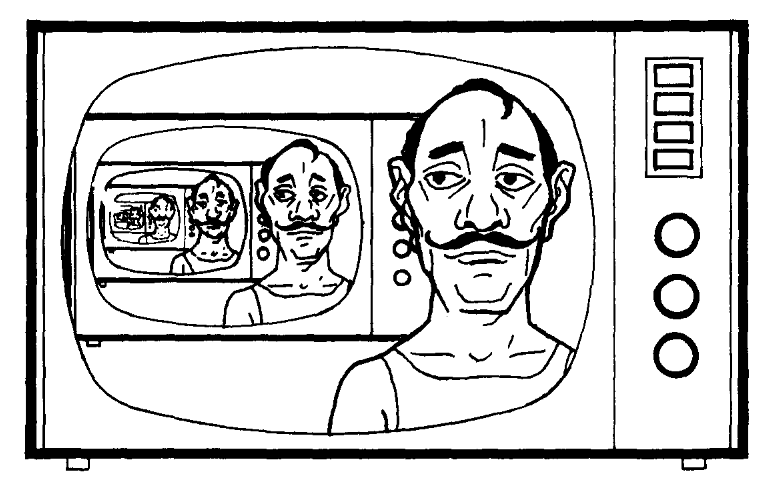
\includegraphics[width=2cm]{images/rec_wirt}}$
        
        $20677=23.$$\stackrel{899}{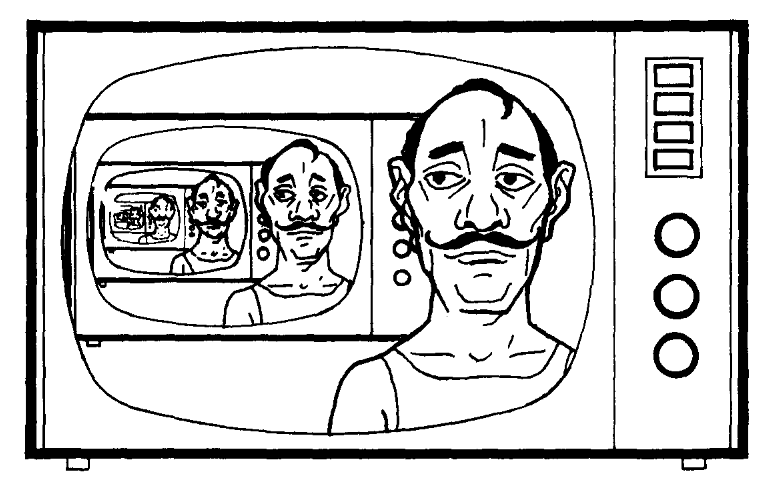
\includegraphics[width=1.6cm]{images/rec_wirt}}$
        
        $899=29.$$\stackrel{31}{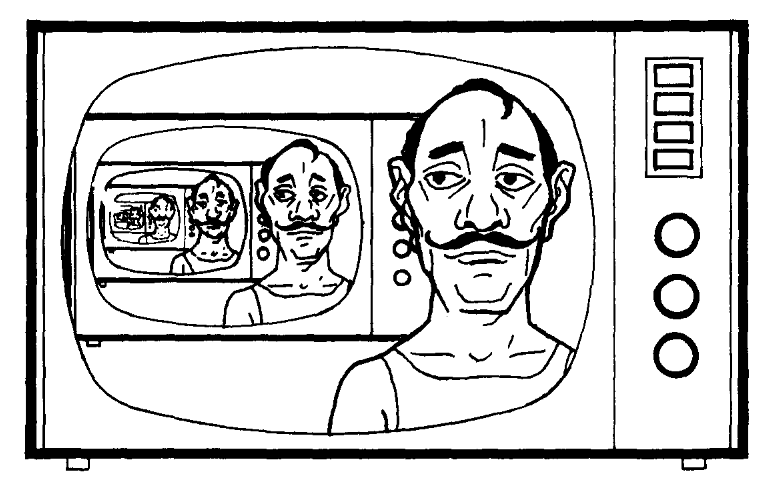
\includegraphics[width=1.2cm]{images/rec_wirt}}$
        
        ...    
      \end{flushright}
      \relscale{1}
      
    \end{column}
  \end{columns}
  
\end{frame}


\begin{frame}[fragile]
  \frametitle{Разлагане на прости делители}

  $351509=17.$$\stackrel{20677}{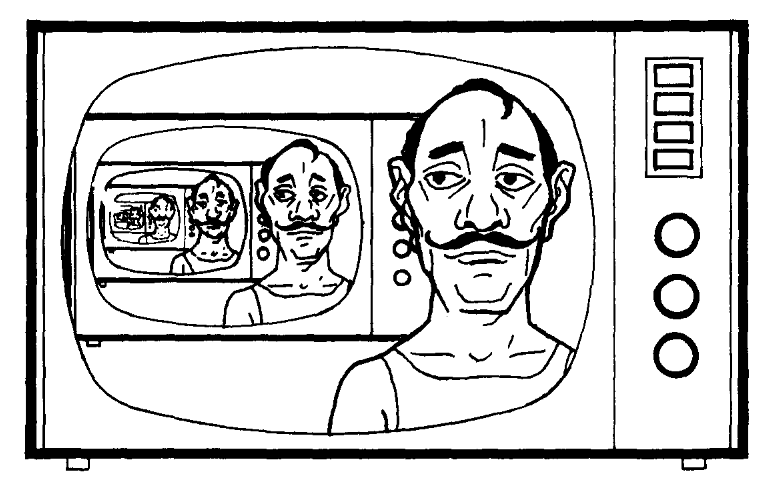
\includegraphics[width=2cm]{images/rec_wirt}}$

\bigskip

\begin{lstlisting}[basicstyle=\small,language=Haskell]
divisors 1 = []
divisors x = fistdivisor x : 
             divisors (div x (fistdivisor x))      
\end{lstlisting}

  
\end{frame}


\begin{frame}[fragile]
  \frametitle{Бързо сортиране}

  \begin{center}
    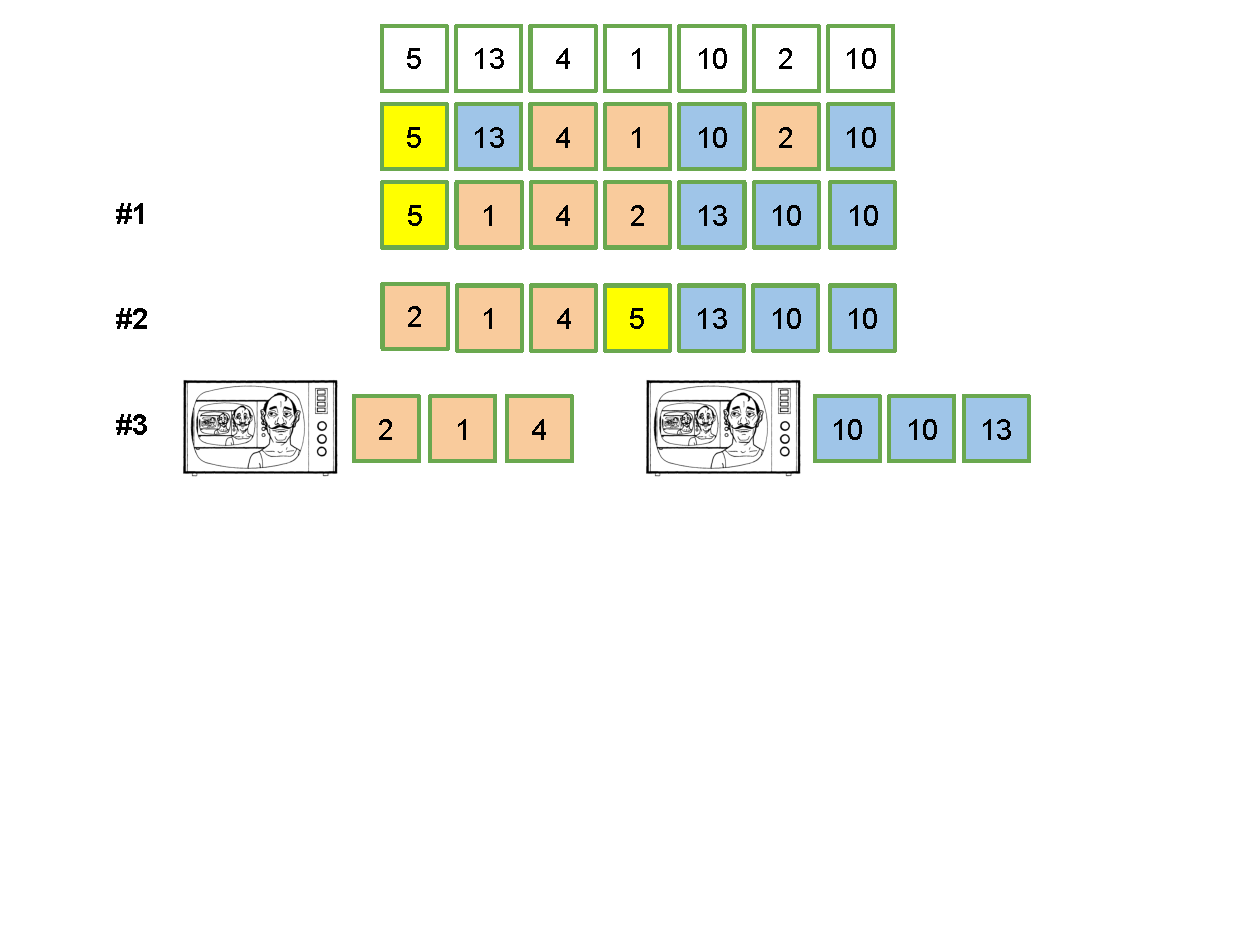
\includegraphics[width=12cm]{images/qsort}
 \end{center}
   
\end{frame}

\vspace*{-0.5cm}


\begin{frame}[fragile]
  \frametitle{Бързо сортиране}

  \begin{center}
    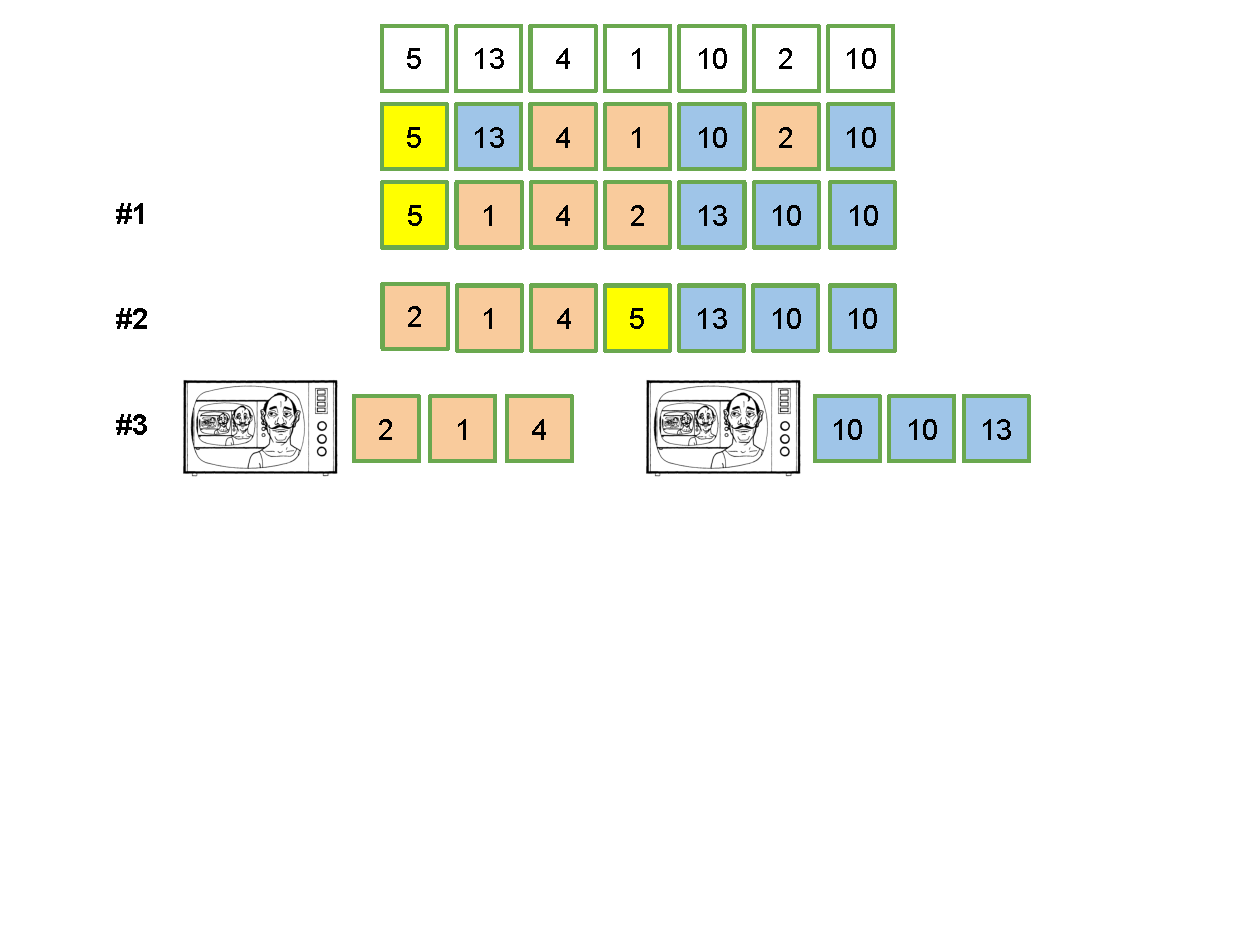
\includegraphics[width=6cm]{images/qsort}
 \end{center}
   
\vspace*{-2cm}

\begin{lstlisting}[basicstyle=\small,language=Haskell]
  split [] _ = ([], [])
  split (x:xs) pivot 
      | x < pivot = (x:smaller, larger)
      | otherwise = (smaller, x:larger)
      where (smaller, larger) = split xs pivot
  
  qsort [] = []
  qsort (x:xs) = qsort smaller ++ [x] ++ qsort larger
      where (smaller, larger) = split xs x
  \end{lstlisting}
  

\end{frame}


\begin{frame}
  \centerline{Търсене на път в лабиринт}
\end{frame}



\begin{frame}[fragile]
  \frametitle{Задачата}
  %\vspace*{-25pt}
  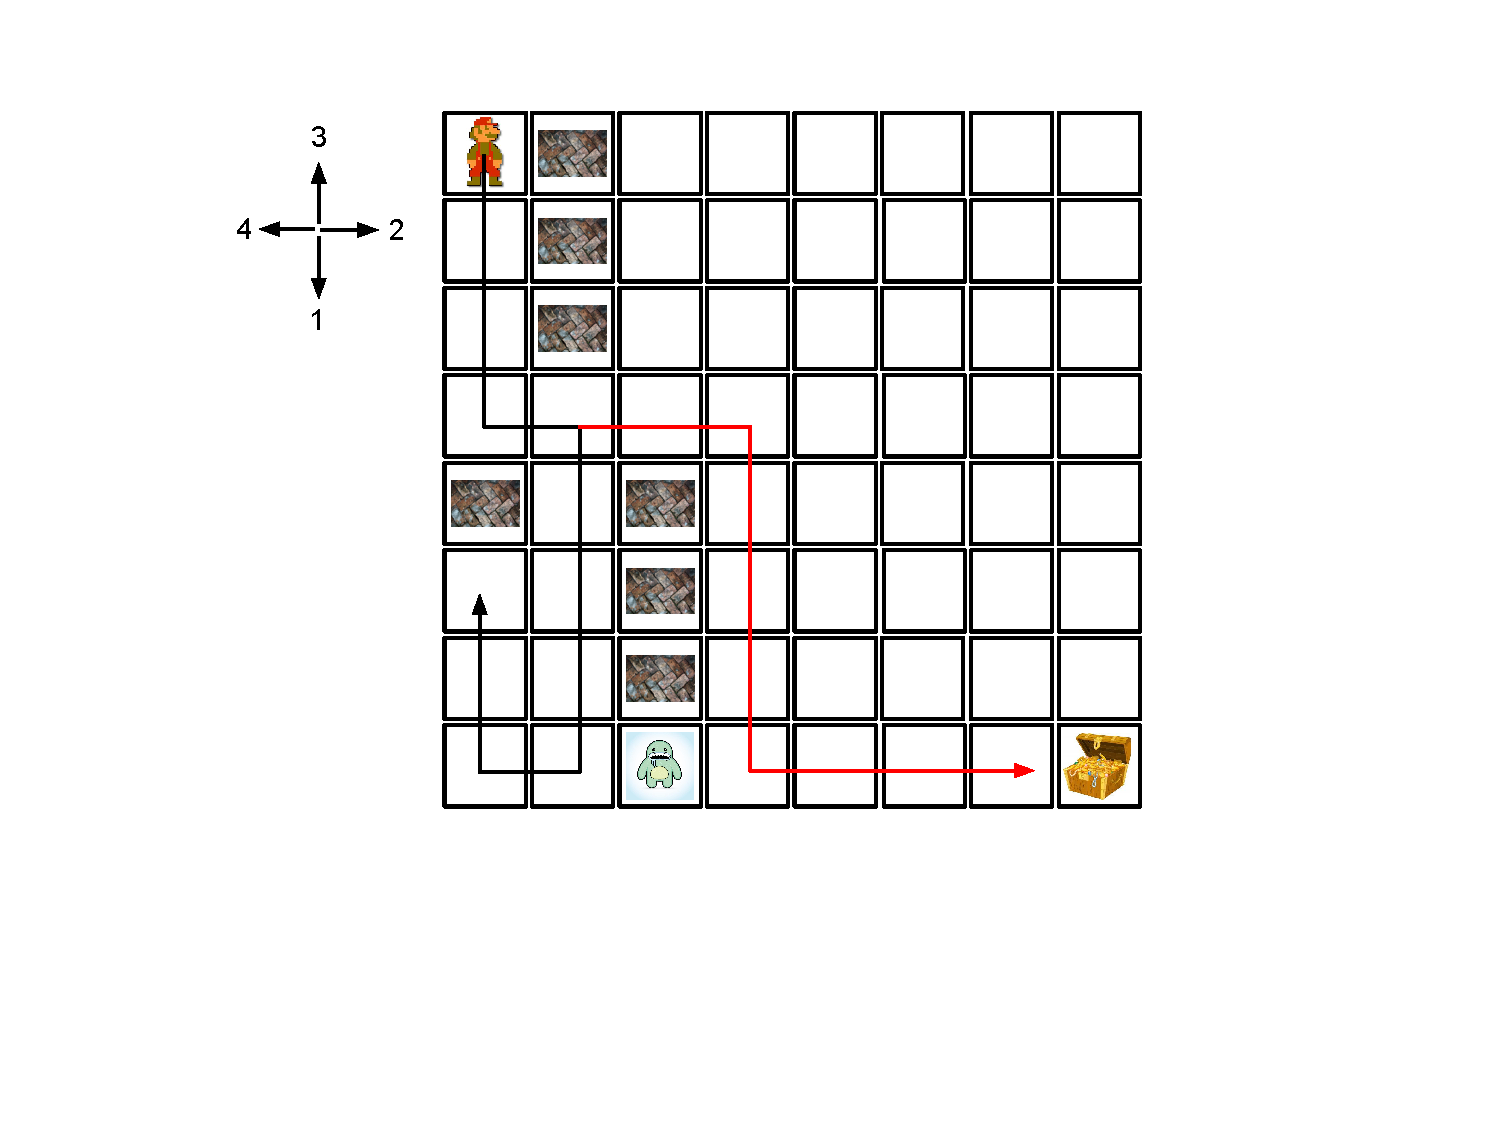
\includegraphics[width=12cm]{images/lab_sol}
\end{frame}

\begin{frame}[fragile]
  \frametitle{Търсене}
  %\vspace*{-25pt}
  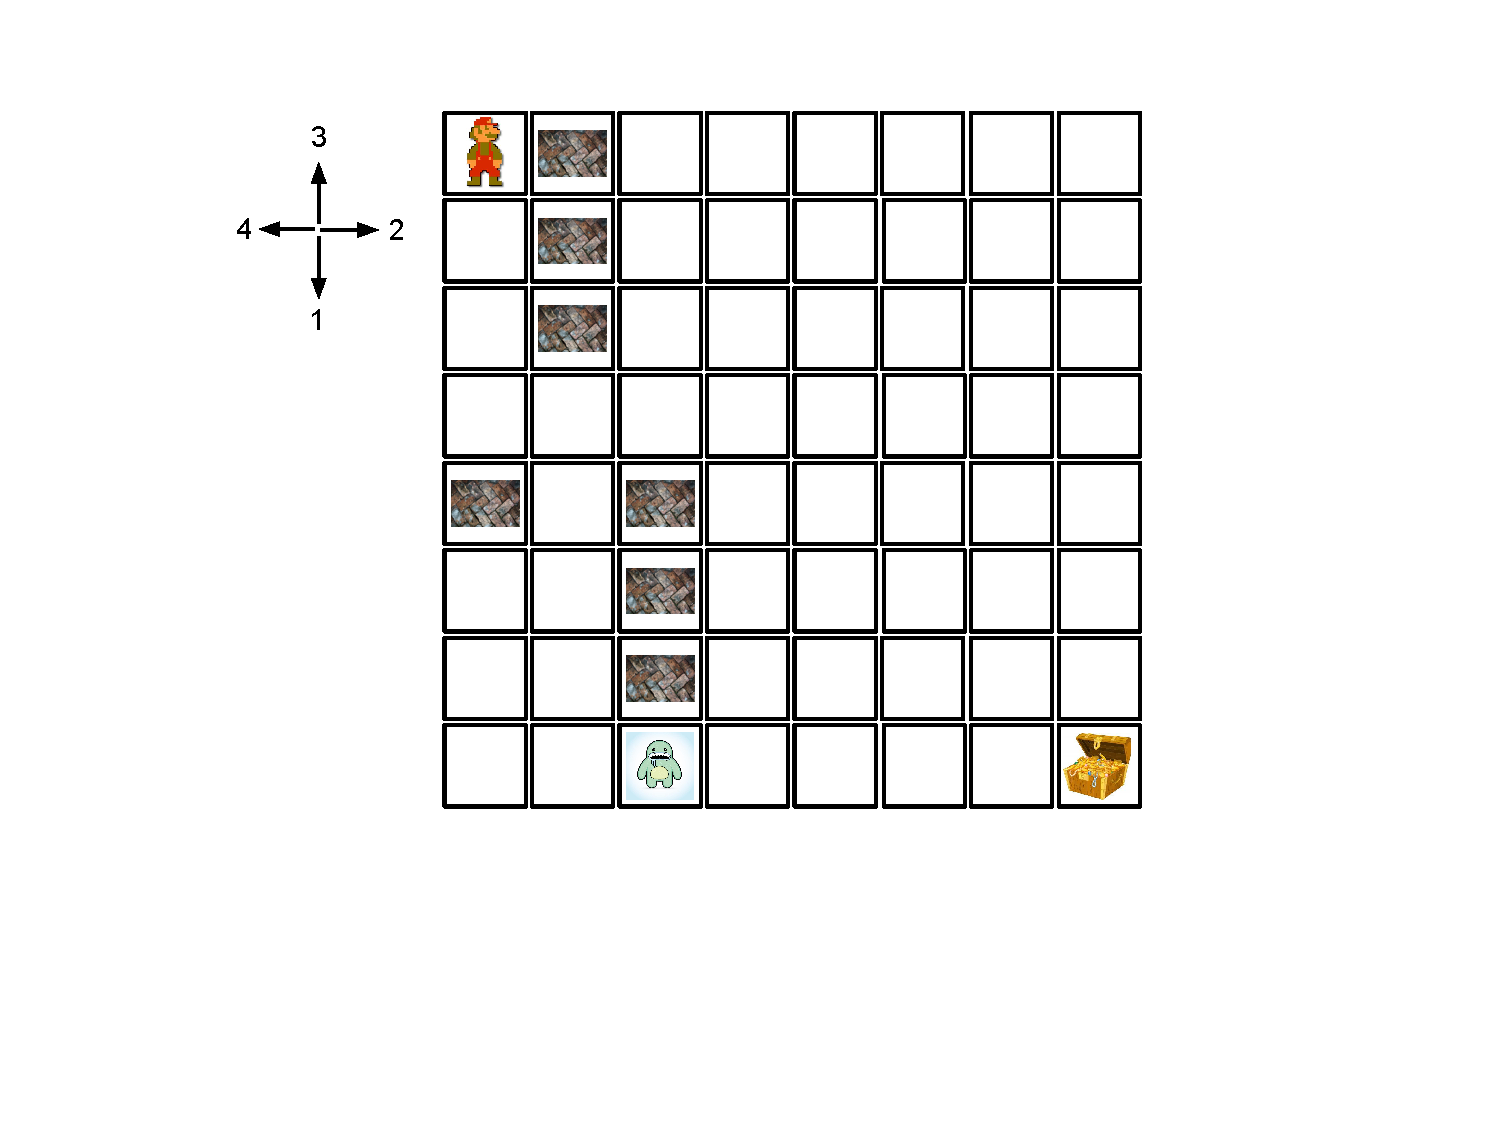
\includegraphics[width=12cm]{images/lab_00}
\end{frame}

\begin{frame}[fragile]
\frametitle{Търсене}
%\vspace*{-25pt}
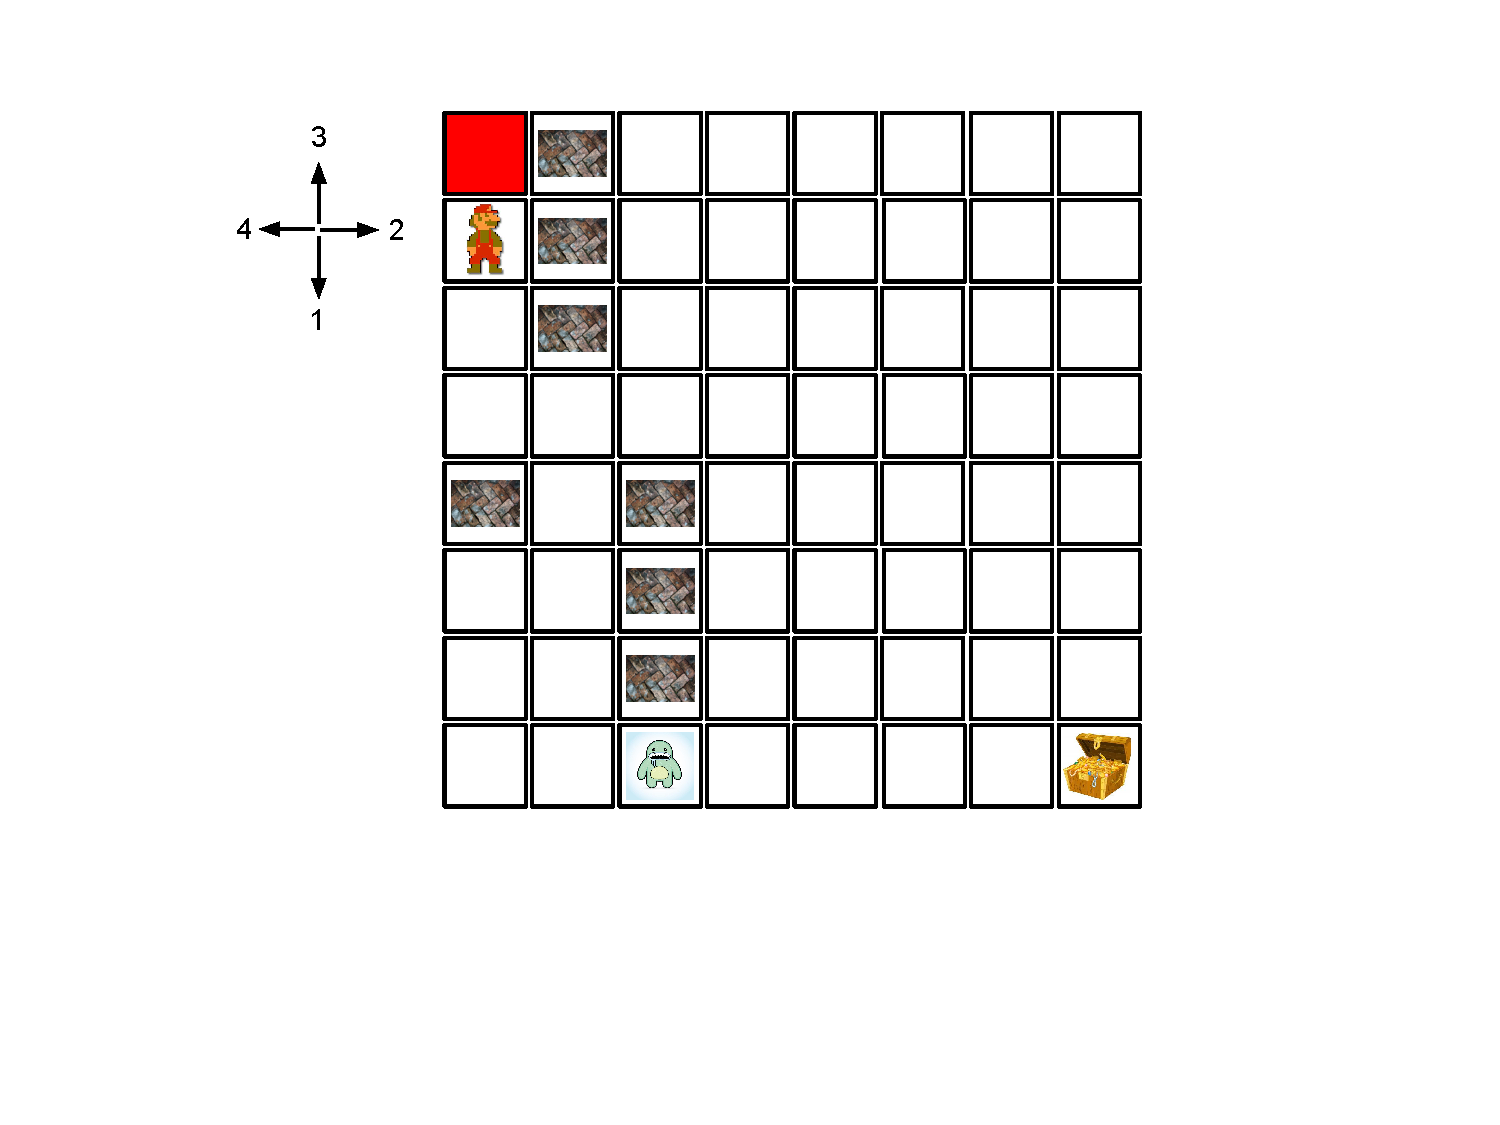
\includegraphics[width=12cm]{images/lab_01}
\end{frame}

\begin{frame}[fragile]
\frametitle{Търсене}
%\vspace*{-25pt}
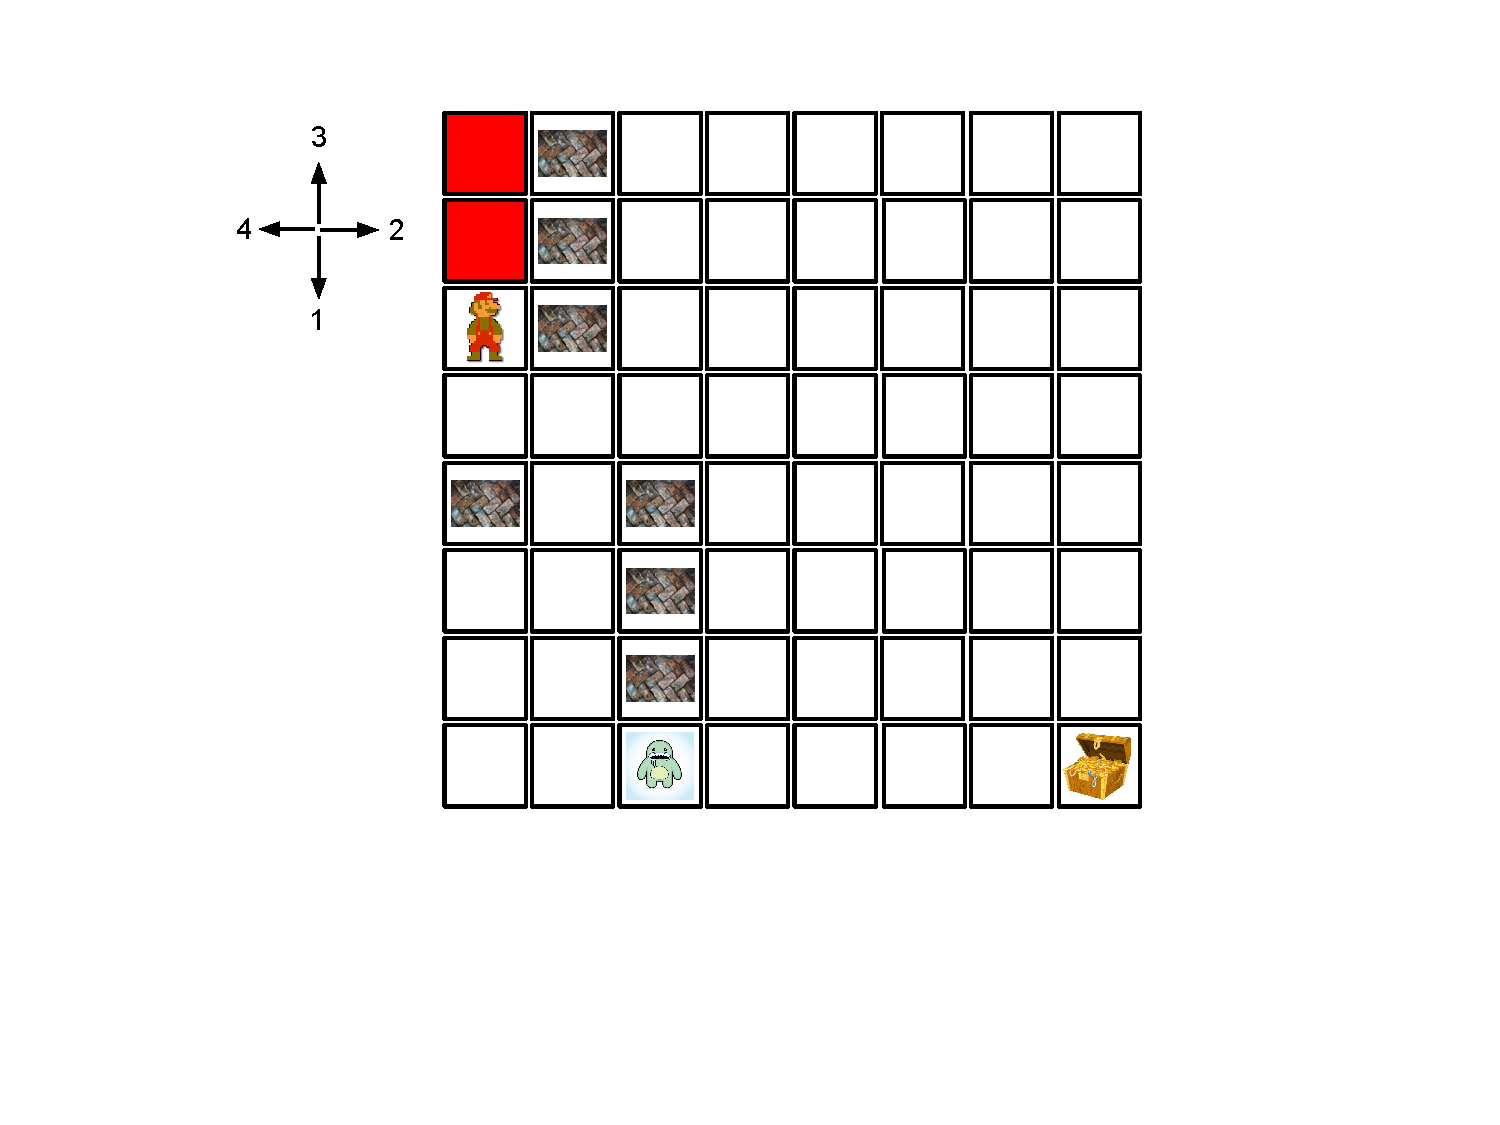
\includegraphics[width=12cm]{images/lab_02}
\end{frame}


\begin{frame}[fragile]
\frametitle{Търсене}
%\vspace*{-25pt}
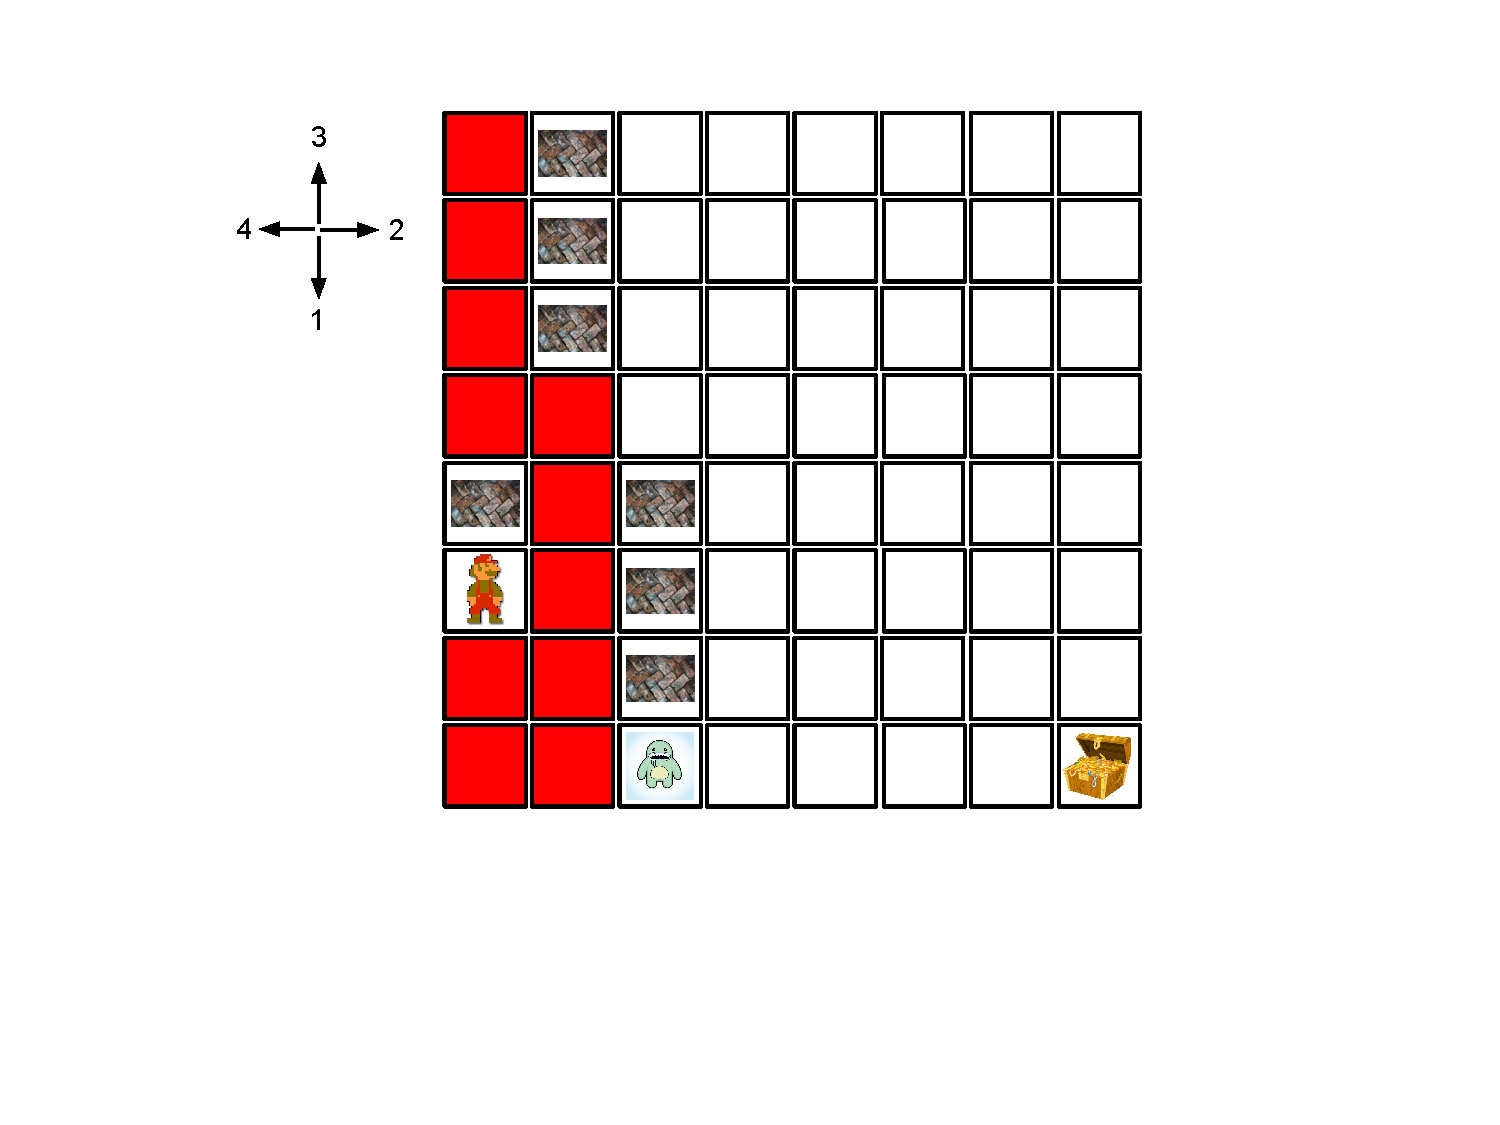
\includegraphics[width=12cm]{images/lab_dead1}
\end{frame}



\begin{frame}[fragile]
\frametitle{Търсене}
%\vspace*{-25pt}
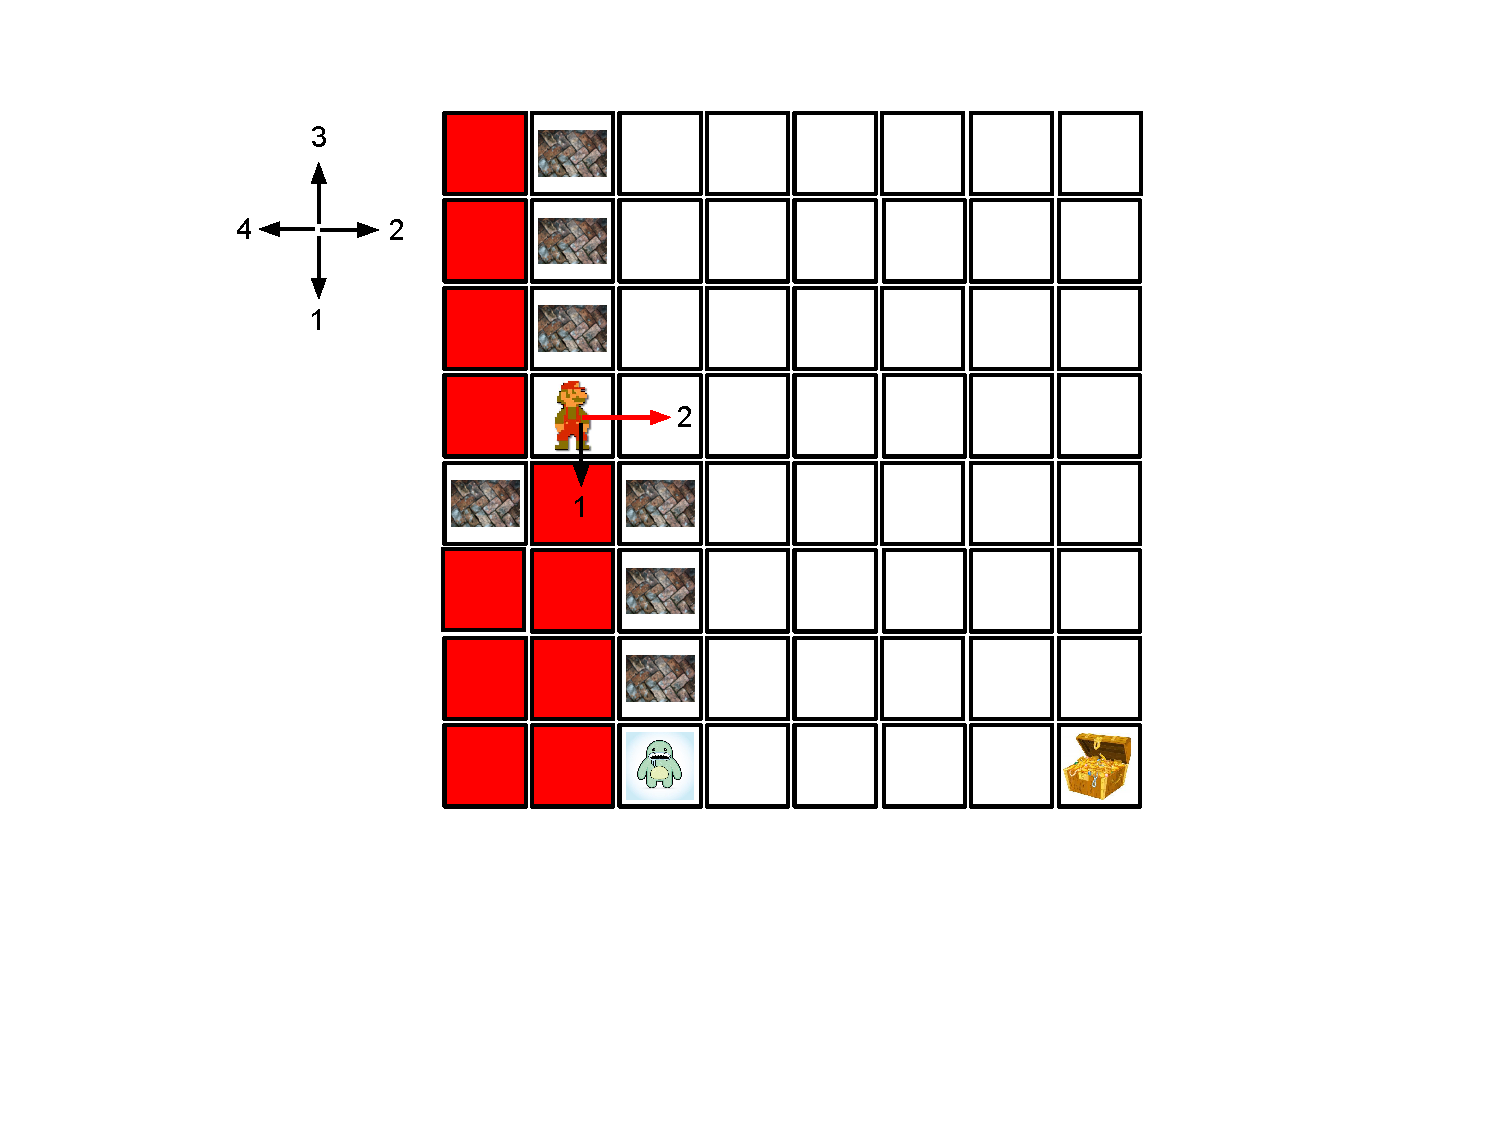
\includegraphics[width=12cm]{images/lab_choice_01}
\end{frame}
  


\begin{frame}[fragile]
  \frametitle{Пълно изчерпване}


\begin{tikzpicture}[remember picture,overlay]
  \node[xshift=80mm,yshift=-12mm,anchor=north west] at (current page.north west){%
  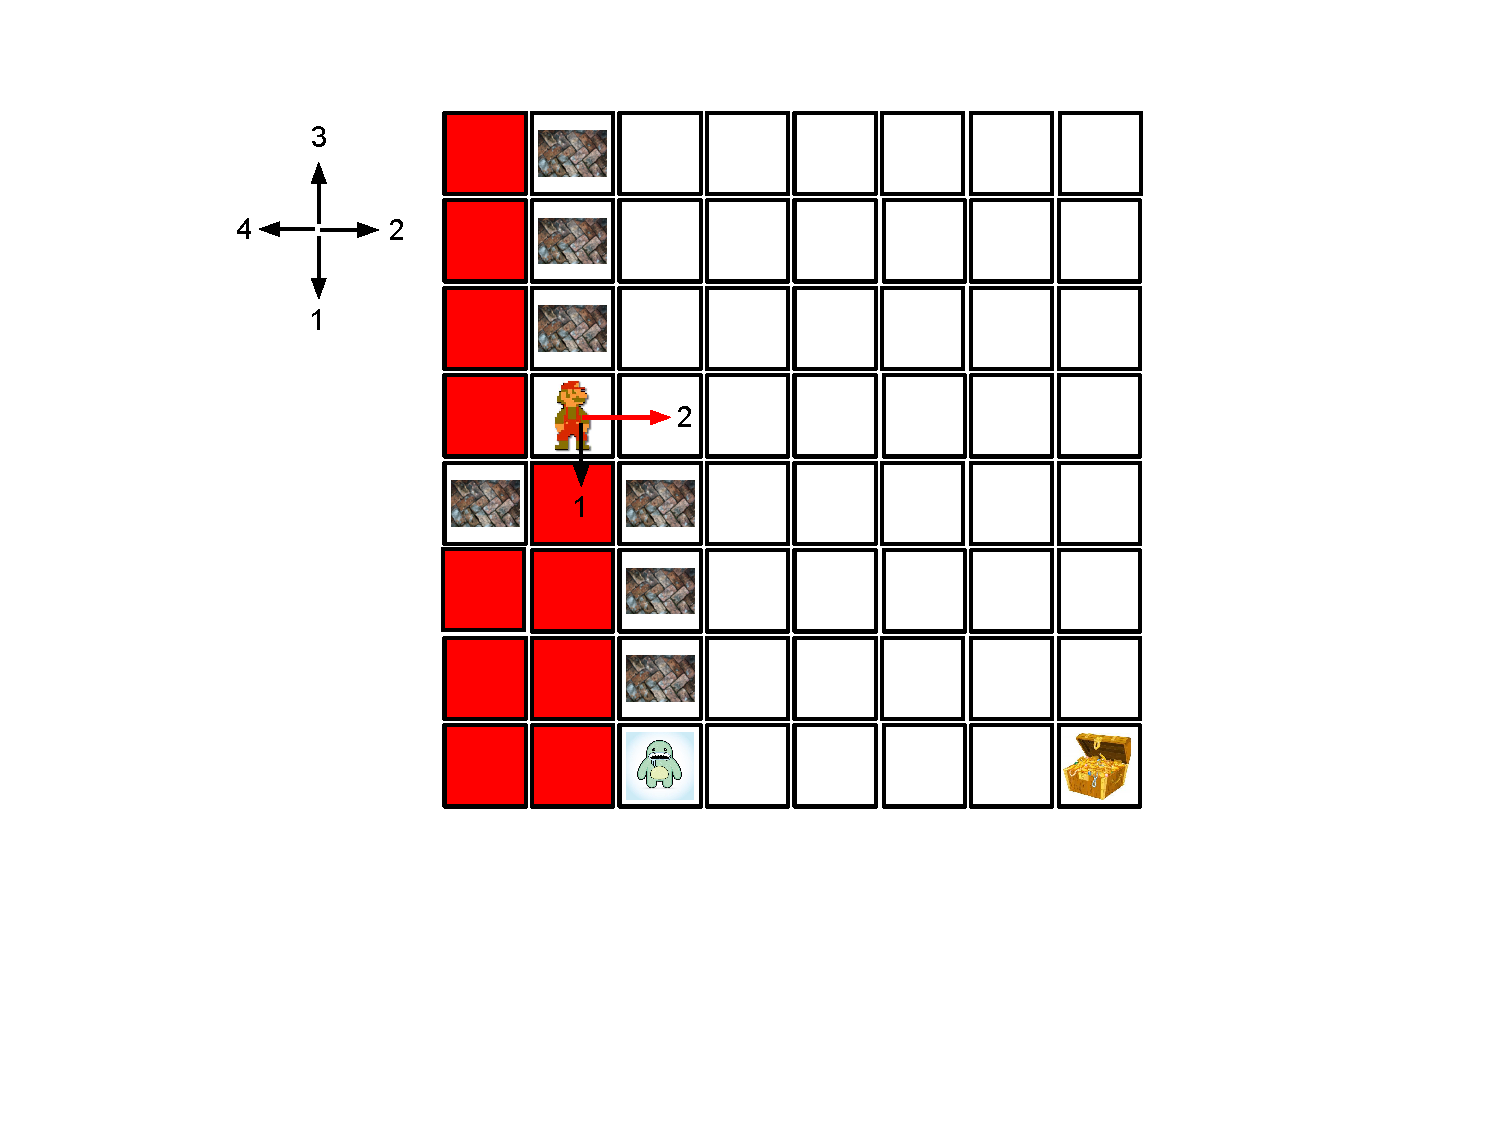
\includegraphics[width=55mm]{images/lab_choice_01}};
\end{tikzpicture}
     
\begin{itemize}
  \item Не е елегантно, засега върши работа
\end{itemize}

\begin{lstlisting}[basicstyle=\small,language=Haskell]
  --findGold :: game visited -> path
  findGold :: Maybe Game -> [Pos] -> [Pos]
  findGold Nothing _ = []
  findGold (Just g@(Game p w)) visited
      | foundGold g = [p]
      | (stuck g) || (elem p visited) = []
      | downpath /= [] = p : downpath
      | rightpath /= [] = p : rightpath
      | uppath /= [] = p : uppath
      | leftpath /= [] = p : leftpath
      where downpath = findGold (down g) (p:visited)
            rightpath = findGold (right g) (p:visited)
            uppath = findGold (up g) (p:visited)
            leftpath = findGold (left g) (p:visited)  
\end{lstlisting}
  

\end{frame}



\end{document}


\begin{columns}[t]
  \begin{column}{0.2\textwidth}

\relscale{0.63}
\begin{lstlisting}
\end{lstlisting}
\relscale{1}

  \end{column}
  \begin{column}{0.8\textwidth}

  \end{column}
\end{columns}


